\documentclass[a4paper, 11pt]{article}

\usepackage[utf8]{inputenc}
\usepackage[frenchb]{babel}
\usepackage[T1]{fontenc}
\usepackage{textcomp}
\usepackage{amsmath,amssymb}
\usepackage{lmodern}
\usepackage[a4paper]{geometry}
\usepackage{graphicx}
\usepackage{xcolor}
\usepackage{microtype}
\usepackage{listings}
\usepackage{hyperref}

\renewcommand*{\familydefault}{\sfdefault}

\title{Aide à la décision}
\author{Dragibus}
\date{}

\begin{document}
\maketitle
\tableofcontents
\newpage

\section{Introduction}
Dans le cadre de notre étude sur l'optimisation quantitative et qualitative
pour le développement valorisé de vos produits, nous avons scindé votre
problématique en trois sections. \\
Dans un premier temps, nous étudierons objectivement les critères opérationnels
proposés par vos cadres pour maximiser vos performances tant en matière de
production qu'en qualité sur le long terme. \\
Ensuite, nous établissons la synergie entre les critères précédemment cités.
Cela amène à une totale compréhension et une vision globale des solutions
envisagées. Par cela, nous entendons placer un compromis pour chacun des
responsables concernés. \\
La dernière partie consistera en l'étabissement d'une solution finale parmi
celles proposées précédemment.

\subsection{Définition}
Nous définissons ici les notations que nous utiliserons dans la suite de ce
rapport et exprimmons certaines notions sous forme de fonctions mathématiques.
\\
Soit $E_M = \left\{1, 2, 3, 4, 5, 6, 7\right\} $ l'ensemble des machines. \\
Soit $E_{MP} = \left\{MP1, MP2, MP3\right\} $ l'ensemble des matières premières. \\
Soit $E_P = \left\{A, B, C, D, E, F\right\} $ l'ensemble des produits. \\
Soit $B$ le bénéfice de l'entreprise. \\
Soit $TTH$ le temps de travail hebdomadaire. \\
Soit $X(i)$ le nombre de produit $i\in E_P$ fait. \\
Soit $X = \left\{X(1), X(2), X(3), X(4), X(5), X(6), X(7)\right\}$ le vecteur
définissant les quantités de chaque produit à fabriquer.\\
Soit $S(p)$ la quantité en stock de la matière première $p\in E_{MP}$. \\
Soit $TM(m)$ le temps d'utilisation de la machine $m\in E_M$.\\
Soit $G(i)$ le gain engendré par le produit $i$. \\
Soit $V(i)$ le prix de vente du produit $i$. \\
Soit $P(i)$ la perte engendrée par le produit $i$. \\
Soit $Q(i, p)$ la quantité de matière $p$ nécessaire pour le produit $i$. \\
Soit $A(p)$ le prix d'achat de la matière $p$. \\
Soit $C(m)$ le cout de la machine $m$. \\
Soit $T(i, m)$ le temps d'usinage de la machine $m$ pour le produit $i$. \\

$$
\begin{array}{r l}
    G(i) =  & V(i)\cdot X(i) \\
    P(i) =  & X(i)\left(\sum_{p\in E_{MP}} A(p)Q(i, p)+ \sum_{m\in E_M} C(m)T(i, m)\right) \\
    B =     & \sum_{i\in E_P} G(i) - P(i) \\
    TM(m) = & \sum_{i\in E_P} X(i)T(i, m) \\
    TTH =   & \sum_{m\in E_M} TM(m) \\
    S(p) =  & \sum_{i\in E_P} X(i)Q(i, p) \\
\end{array}
$$

\subsection{Ensemble des contraintes}
Cette section exprime sous forme mathématique les différentes contraintes
inhérentes au fonctionnement de l'entreprise.

$$
\begin{array}{r l}
    \forall i\in E_P, & X(i) > 0 \\
    \forall m\in E_M, & TM(m) \in [0, 4800\mbox{min}] \\
                      & TTH \in [0, 4800\mbox{min}] \\
                      & B > 0 \\
                      & S(MP1) \in [0, 650] \\
                      & S(MP2) \in [0, 820] \\
                      & S(MP3) \in [0, 585] \\
\end{array}
$$

\section{Optimisation monocritère}
Dans cette partie, nous considérons un par un les différents critères retenus
par les différents cadres de l’entreprise ADécision. Nous commençons par
exprimer le problème sous forme d’un modèle mathématique. Il est possible de
modéliser chacune des situations suivantes sous forme d’une fonction $f$ de $X$ à
minimiser en respectant la condition $A . X \leq b$. \\

\begin{minipage}[c]{.49\linewidth}
    \centering
    $A = \begin{pmatrix}
        11&15&0&5&0&10 \\
        0&1&2&8&7&12\\
        12&1&11&0&10&15\\
        2&10&5&4&13&7\\
        15&0&0&0&10&25\\
        5&5&13&12&8&0\\
        5&3&5&28&0&7\\
        1&1&1&5&0&2\\
        2&2&1&0&2&1\\
        1&0&3&2&6&0
    \end{pmatrix}$\\
\end{minipage}
\hfill
\begin{minipage}[c]{.49\linewidth}
    \centering
    $b = \begin{pmatrix}
        4800\\
        4800\\
        4800\\
        4800\\
        4800\\
        4800\\
        4800\\
        650\\
        820\\
        585\\
    \end{pmatrix}$
\end{minipage}

\subsection{Comptable}
L'objectif du comptable est de maximiser les bénéfices de l'entreprise.
Il suffit donc de maximiser la fonction de bénéfice définie précédemment.

$G(X) = X\cdot(28~20~30~37~45~22)^t$ \\

$$
\begin{array}{r l}
    \mbox{CoutAchat}(A) = & (1~2~1)\cdot(3~4~2)^t = 13 \\
    \mbox{CoutAchat}(B) = & (1~2~0)\cdot(3~4~2)^t = 11 \\
    \mbox{CoutAchat}(C) = & (1~1~3)\cdot(3~4~2)^t = 13 \\
    \mbox{CoutAchat}(D) = & (5~0~2)\cdot(3~4~2)^t = 19 \\
    \mbox{CoutAchat}(E) = & (0~2~6)\cdot(3~4~2)^t = 20 \\
    \mbox{CoutAchat}(F) = & (2~1~0)\cdot(3~4~2)^t = 10 \\
\end{array}
$$

$$
\begin{array}{r r l l}
    \mbox{CoupMachine}(A) = & (11~0~12~2~15~5~5)\cdot  & \frac{1}{60}(2~2~1~1~2~3~1)^t = & \frac{86}{60} \\
    \mbox{CoupMachine}(B) = & (15~1~1~10~0~5~3)\cdot   & \frac{1}{60}(2~2~1~1~2~3~1)^t = & \frac{61}{60} \\
    \mbox{CoupMachine}(C) = & (0~2~11~5~0~13~5)\cdot   & \frac{1}{60}(2~2~1~1~2~3~1)^t = & \frac{64}{60} \\
    \mbox{CoupMachine}(D) = & (5~8~0~4~0~12~28)\cdot   & \frac{1}{60}(2~2~1~1~2~3~1)^t = & \frac{94}{60} \\
    \mbox{CoupMachine}(E) = & (0~7~10~13~10~8~0)\cdot  & \frac{1}{60}(2~2~1~1~2~3~1)^t = & \frac{71}{60} \\
    \mbox{CoupMachine}(D) = & (10~12~15~7~25~0~7)\cdot & \frac{1}{60}(2~2~1~1~2~3~1)^t = & \frac{123}{60} \\
\end{array}
$$

$$
\begin{array}{r l}
    P(X) = & X\cdot\left((13~11~13~19~20~10) + \frac{1}{60}(86~61~64~94~71~123)\right)^t \\
    = & X\cdot\frac{1}{60}(866~721~844~1234~1271~723)^t \\
\end{array}
$$

$$
\begin{array}{r l}
    B(X) = & G(X) - P(X) \\
    = & X\cdot\frac{1}{60}(814~479~956~986~1429~597)^t \\
    = & X\cdot(13.5667~7.98333~15.9333~16.4333~23.8167~9.95)^t \\
\end{array}
$$

L'on détermine donc le vecter X maximisant les bénéfices selon les contraintes du problème en minimisant la fonction :\\
$$
\begin{array}{rl}
    f(X) = & -B(X) \\
    = & X\cdot(-13.5667~-7.98333~-15.9333~-16.4333~-23.8167~-9.95)^t
\end{array}
$$

sous les contraintes
$$
\left\{\begin{split}
    A\cdot X \leq b\\
    0 \leq X
\end{split}\right.
$$

L'on obtient le résultat suivant : \\
$ X = (235.6250~98.3929~101.3393~22.6786~0~50.6280) $ \\

Cela correspond à un bénéfice de 6473.2 €.

\subsection{Responsable d'atelier}
L'objectif du responsable atelier est de maximiser le nombre de produits fabriqués.
Il faut donc minimiser la fonction suivante : \\
$$
\begin{array}{rl}
    f(X) = & -X(A) + -X(B) + -X(C) + -X(D) + -X(E) + -X(F) \\
    = & X\cdot(-1~-1~-1~-1~-1~-1)^t
\end{array}
$$

en respectant les contraintes suivantes : \\
$$
\left\{\begin{split}
    A\cdot X \leq b\\ 
    0 \leq X
\end{split}\right.
$$

L'on obtient le résultat suivant : $ X = (0~252.5~195.0~0~0~101.25) $ \\

\subsection{Responsable commercial}
L'objectif du responsable commercial est d'équilibrer les quantités faites par famille de produits.
La quantité de production des produits A, B et C doit être la même que celle des produits D, E et F : \\
$X(A) + X(B) + X(C) = X(D) + X(E) + X(F)$ \\

La fonction a minimiser est donc celle représentant la différence de production des deux familles : \\
Si l’on souhaite maximiser la production tout en respectant la contrainte que nous
nous sommes fixés précédemment, on réutilise la fonction $f$ utilisée par le
responsable d’atelier : $ f(X) = X\cdot(1~1~1~1~1~1)^t $

On utilise alors le meme procédé qu'avec le responsabme d'atelier en ajoutant
la contrainte précédemment trouvé représenté par l'équation : \\
$ f_c(X) = 0, f_c(X) = X\cdot(1~1~1~-1~-1~-1)^t $.

On trouve alors comme solution $X = (0~206.03~43.26~14.70~70.97~163.6) $ \\

Si l’on souhaite maximiser les bénéfices tout en respectant l’objectif que nous
nous sommes fixés précédemment, on réutilise la fonction $f$ utilisée par le
comptable. On trouve alors le meme $X$ qu'avant. \\

On peut donc voir que, en maximisant le bénéfice, ou en maximisant le nombre de
pièces produites, le fait d’égaliser le nombre de produits par famille fait
converger les deux résultats. On trouve un bénéfice de 5893,8 unités d’argent,
ce qui correspond à 91,05\% du bénéfice maximal.

\subsection{Responsable des stocks}
Le responsable des stocks veut minimiser la taille des stocks, c'est à dire le
nombre de produits ainsi que la quantité de matières premières stockée. On
cherche également à garder un bénéfice positif permettant à l'entreprise de
continuer sa croissance. On considère alors la taille de stock initial au début
de la semaine de production plus l'espace que prendront les produits fabriqués.

La fonction à minimiser est donc la suivante : \\
$$
\begin{array}{rl}
    f(X) = & 2\cdot \sum_{p\in E_{MP}} S(p) \\
    = & 5 X(A) + 6 X(B) + 8 X(D) + 9 X(E) + 4 X(F) \\
    = & X\cdot(5~6~8~9~4)^t
\end{array}
$$

Le stock ne peut être négatif on le contraint donc à être supérieur à 0. Le
minimum de cette fonction est alors 0. Or l'entreprise doit toujours pouvoir
produire. Il est ainsi nécessaire de rajouter des contraintes afin d'avoir un
résultat réaliste. On contraint le système en prenant alors d'autres
critères. On peut maximiser le bénéfice ou la production par exemple. Nous
avons choisi de traduire l’activité de l’entreprise grâce à son bénéfice. \\

\textbf{TODO rajouter l'image qu'il y a sur le drive
+ donner une explication (donc changer un peu le paragraphe suivant} \\

La solution est considérée comme viable si le bénéfice est au moins supérieur à
70\% du bénéfice total. On remarque un point d’inflection pour un stock de
407.2 unités correspondant à un bénéfice de 5742 unités d’argent (soit 88.7\% du
bénéfice maximum). Il n’est donc pas judicieux de chercher une solution avec
un bénéfice plus élévé car cela entrainerait une augmentation beaucoup plus
rapide des stocks. \\

On trouve alors : $ X = (319.5453 ~0.3081 ~87.1207 ~0.0000 ~0.6821 ~0.0000) $

\subsection{Responsable du personnel}
L’objectif du responsable du personnel est de minimiser le temps d’utilisation
des machines 1 et 5 pour l’ensemble de la production. Alors, il s’agit de
minimiser la fonction suivante:\\

$$
\begin{array}{rl}
    f(X) = & (TM1A + TM5A)\cdot X(A) \\
           & + (TM1B + TM5B)\cdot X(B) \\
           & + (TM1C + TM5C)\cdot X(C) \\
           & + (TM1D + TM5D)\cdot X(D) \\
           & + (TM1E + TM5E)\cdot X(E) \\
           & + (TM1F + TM5F)\cdot X(F) \\
    = & 26X(A) + 15X(B) + 0X(C) + 5X(D) + 10X(E) + 35X(F) \\
    = & X\cdot (26~15~0~5~10~35)^t
\end{array}
$$

La table des temps de production d’un produit par machine nous montre, que le
produit C n’a pas besoins des deux machines en question, ce qui signifie que la
solution la plus simple est d’arreter la production des autres produits et de
se concentrer sur la fabrication du produit C. \\
Une approche algorithmique confirme cette solution et nous donne le plan de
production suivant: $X = (0 ~0 ~135.6644 ~0 ~0 ~0)$ \\

Par contre, cette solution ne donne pas assez de bénéfice pour l’entreprise, il
faut alors ajouter d’autres contraintes afin de trouver une vraie solution.
Tenant en compte le bénéfice de l’entreprise, on souhaite ne pas souspasser
70\% du bénéfice maximum. Si on considère cette nouvelle contrainte et qu’on
calcule le montant des produits à fabriquer, on obtient le graphique
(fig. \ref{fig_graph_personnel_temps}).

\begin{figure}[position]
    \begin{center}
        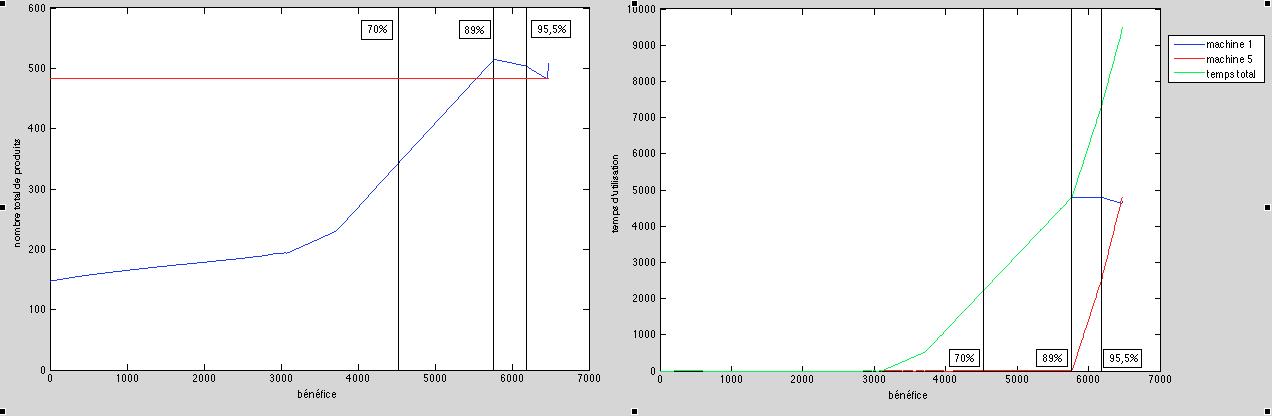
\includegraphics[scale=0.35]{graph_personnel_temps}
        \caption{
            \label{fig_graph_personnel_temps} Legende de l'image (à faire ?).
        }
    \end{center}
\end{figure}

Pour respecter les 70\% du benefice maximum, l’entreprise doit fabriquer un
total de 343.1 produits. Par contre, le deuxième graphique nous montre que la
machine 5 n’est pas du tout utilisée jusqu’aux 89\%. Puisqu’on souhaite
utiliser les deux machines, on choisit un plan de production correspondant à
95,5\% pour raison de changement de la dérivée de la fonction du temps
d’utilisation de la machine 5 à ce point-là. \\

Donc le plan de production est le suivant: \\
$X = (168 168.7394~ 184.0703~ 114.3787~ 36.5623~ 0.0000~ 0.0000)$

\section{Programmation linéaire multicritère}
\subsection{Matrice de Gain}

La matrice de gain, correspondant aux valeurs clés, prises dans le cas
idéal de chaque responsable, est générée à partir des choix d'une
programmation mono-critères. \\

% TODO mettre une référence vers le mono-critère au lieu de ça
Prenant les stratégies de production pour chaque responsable comme suit :

\begin{itemize}
    \item Xcomptable = [235.625; 98.3929; 101.3393; 22.6786; 0; 50.625]
    \item Xcommercial = [0; 206.03; 43.26; 14.7; 70.97; 163.61]
    \item Xatelier = [0; 252.5; 195; 0; 0; 101.2500]
    \item Xstocks = 1.0e-16 * [0.5614; 0.2369; 0.114; 0.0365; 0.0028; 0.2099]
    \item Xpersonnel = [0; 0; 135.6644; 0; 0; 0]
\end{itemize}

Et retenant les anciennes fonctions à optimiser, on trouve :

$$
G =
\left (
    \begin{array}{ccccc}
        6473.2 & 362.1 & 508.7 & 2563.7 & 9487.4 \\
        5893.8 &     0 & 498.6 & 2494.4 & 9600.0 \\
        6130.2 & 346.3 & 548.7 & 2585.0 & 7331.2 \\
        0 &     0 &     0 &      0 &      0 \\
        2161.6 & 135.7 & 135.7 &  814.0 &      0
    \end{array}
\right )
$$

Les colonnes de cette matrice correspondent aux point de vues associés à chaque
responsable, c'est à dire la valeur lui important, il peut s'agir d'euros ou
d'unités produites, selon le responsable concerné. Les lignes quand à elles
correspondent à des stratégies de production à suivre, prises pour chaque
responsable, dans le même ordre que les colonnes. \\

On remarque que les valeurs se trouvant sur la diagonale correspondent à des
maximums/minimums, en l'occurence des optimums. Ceci confirme la validité de
la matrice de gain, car chaque responsable se trouve dans "son" cas optimal
à cet endroit.

\subsection{Équilibrage inter-critères}

En considérant le bénéfice comme variable "clé" intervenant dans ce problème,
l'optimisation des solutions se fait en procédant à une interpolation linéaire
entre le cas générant le plus de bénéfices, et le cas idéal pour chaque
responsable. \\

% TODO réparer le positionnement de l'image
%\begin{figure}
%    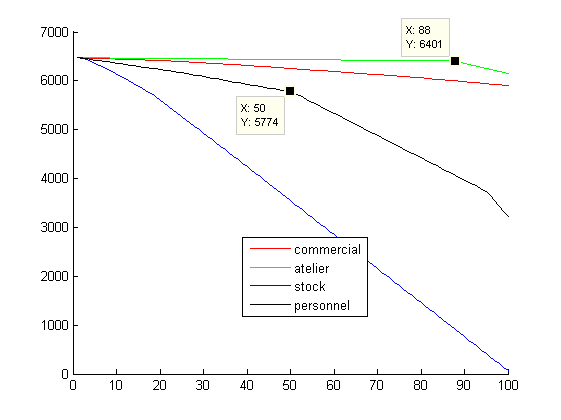
\includegraphics{graph_multi.png}
%    \caption{Graphe représentant l'évolution du bénéfice (en euros) par
%             rapport au pourcentage d'interpolation linéaire.}
%\end{figure}

Nous pouvons noter que les critères du responsable d'atelier et du responsable
commercial n'influent pas énormément sur le bénéfice, contrairement au
responsable des stocks, qui présente une corrélation linéaire avec la
diminution du bénéfice.
Nous remarquons que l'évolution du bénéfice en fonction du compromis pour les
responsables d'atelier et du personnel démarre par une décroissance faible
jusqu'à certaines valeurs de compromis "critiques" (respectivement 88\% et
50\%), ou la pente de dégression s'accroit. \\

De ce fait, nous ajusterons le compromis de ces derniers à ces valeurs limites,
afin qu'ils soient satisfaits au maximum, sans engendrer une perte trop
importante de bénéfice. \\

% TODO


\section{Analyse multicritère}
Le but de cette analyse multi-critère est de déterminer la meilleure solution
parmis les 8 solutions proposées dans la matrice des jugements qui nous a été
donnée. \\

Comme nous souhaitons faire émerger une solution unique, la meilleure (et non
pas classer les solutions les unes par rapport aux autres) grâce aux critères
qui ont été retenus, nous allons utiliser la méthode de détermination Electre
1. \\

Dans un premier temps dans cette analyse multi-critère, nous avons considéré
que tous les critères étaient de même poids. \\

Nous avons ainsi calculé les matrices de concordance et de discordance
relatives à la matrice de jugement. \\
\begin{figure}
    \begin{center}
        \begin{tabular}{|c c c c c|}
            0&3&3&2&3\\
            1&0&2&2&2\\
            2&2&0&2&3\\
            2&3&2&0&3\\
            2&2&3&1&0\\
        \end{tabular}
        \caption{Matrice de concordance (x4)}
    \end{center}
\end{figure}

\begin{figure}
    \begin{center}
        \begin{tabular}{|c c c c c|}
            10&4&2&4&2\\
            2&10&3&6&1\\
            3&4&10&5&2\\
            3&7&3&10&5\\
            3&3&2&5&10\\
        \end{tabular}
        \caption{Matrice de discordance (x10)}
    \end{center}
\end{figure}

Nous avons par la suite testé différentes solutions que voici : \\

On fait varier les seuils de surclassement ainsi que : \\
\begin{figure}
    \begin{center}
        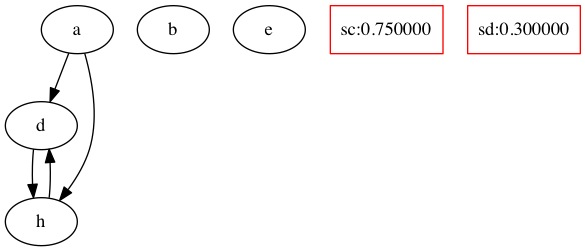
\includegraphics[scale=0.6]{partie3/graph_3_4_3_10.jpeg}
        \caption{Graphe de surclassement : sc = 3/4, sd = 3/10}
    \end{center}
\end{figure}

Avec un seuil de concordance de 3/4 et un seuil de discordance de 3/10, on peut
voir qu’il reste de nombreux liens à faire et donc que les seuils qui ont été
pris sont trop restrictifs. \\

\begin{figure}
    \begin{center}
        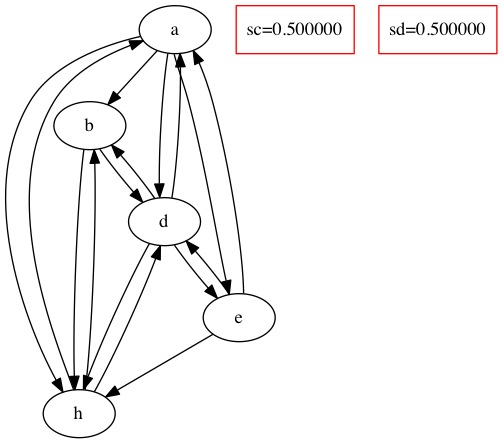
\includegraphics[scale=0.5]{partie3/graph_2_4_5_10.jpeg}
        \caption{Graphe de surclassement : sc = 5/4, sd = 5/10}
    \end{center}
\end{figure}

En prenant un seuil de concordance de 2/4 et un seuil de discordance de 5/10,
on peut voir à l’inverse que trop de liens ont été créés, et la situation est
inexploitable. Nous avons donc choisi des critères trop souples. \\

\begin{figure}
    \begin{center}
        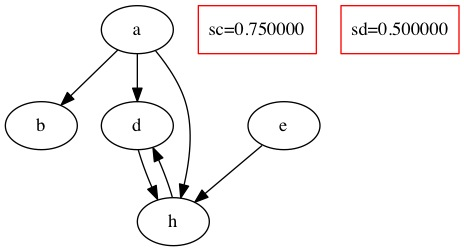
\includegraphics[scale=0.7]{partie3/graph_3_4_5_10.jpeg}
        \caption{Graphe de surclassement : sc = 3/4, sd = 5/10}
    \end{center}
\end{figure}

En prenant un seuil de concordance de 3/4 et un seuil de discordance de 5/10,
on obtient un résultat plus correct cependant elle n’est pas exploitable car
aucune solution ne se dégage clairement, notamment A et E. L’analyse sans
pondération ne suffit donc pas, il va falloir aller plus loin et refaire la
même démarche d’analyse approfondie. \\

Nous allons donc recommencer l’analyse en donnant les poids suivants aux critères : \\
\begin{itemize}
    \item g1 (bénéfice) est de poids 4.
    \item g2 (gestion du stock) est de poids 1.
    \item g3 (équilibre commercial) est de poids 2.
    \item g4 (utilisation des machines 1 et 5) est de poids 2.
\end{itemize}

On met également en place de nouvelles échelles de jugement. \\
Les notes iront de 0 à 10 pour un poids fort (g1), de 2 à 8 pour un poids moyen
(g3 et g4) et de 3 à 7 pour un poids faible (g2). \\

Nous effectuons donc un changement d’échelle sur les notes de la matrice de
jugement : \\
Avec $x\in[a1,b1]$ l’élément de la matrice de jugement dans l’ancienne échelle. \\
~~~~~$y\in[a2,b2]$ l’élément de la matrice de jugement dans la nouvelle échelle. \\
$y = x\cdot(b2-a2)/(b1-a1) + (a2\cdot b1-a1\cdot b2)/(b1-a1)$

De poids fort à poids moyen : $y = x\cdot(8-2)/10 + (2\cdot 10-0)/10 = 0.6\cdot x + 2$ \\
De poids fort à poids faible :$y = x\cdot(7-3)/10 + (3\cdot 10-0)/10 = 0.4\cdot x+ 3$ \\

Cette transformation donne la nouvelle matrice de jugement : \\
\begin{figure}
    \begin{center}
        \begin{tabular}{|c c c c|}
            6&5&5&5\\
            5&4.6&7.4&3.8\\
            3&5.8&5&4.4\\
            5&5.4&3.2&7.4\\
            3&5&6.2&4.4\\
        \end{tabular}
        \caption{Nouvelle matrice de jugement}
    \end{center}
\end{figure}

Nous pouvons calculer les nouvelles matrices de concordance et de discordance : \\
\begin{figure}
    \begin{center}
        \begin{tabular}{|c c c c c|}
            0&7&8&6&7\\
            2&0&6&6&7\\
            3&3&0&3&7\\
            3&6&6&0&7\\
            3&3&8&2&0\\
        \end{tabular}
        \caption{Matrice de concordance (x9)}
    \end{center}
\end{figure}

\begin{figure}
    \begin{center}
        \begin{tabular}{|c c c c c|}
            10&2.4&0.8&2.4&1.2\\
            1.2&10&1.2&3.6&0.6\\
            3&2.4&10&3&1.2\\
            1.8&2.4&1.8&10&3\\
            3&2&0.8&3&10\\
        \end{tabular}
        \caption{Matrice de discordance (x10)}
    \end{center}
\end{figure}

Nous testons une nouvelle fois différentes solutions : \\
\begin{figure}
    \begin{center}
        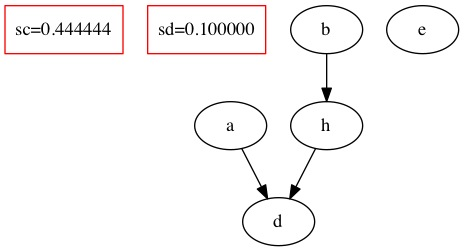
\includegraphics[scale=0.7]{partie3/graph_4_9_1_10.jpeg}
        \caption{Graphe de surclassement : sc = 4/9, sd = 1/10}
    \end{center}
\end{figure}

Comme lors de la première analyse, nous avons pris des seuils trop
contraignants avec un seuil de concordance de 4/9 et un seuil de discordance de
1/10. \\

\begin{figure}
    \begin{center}
        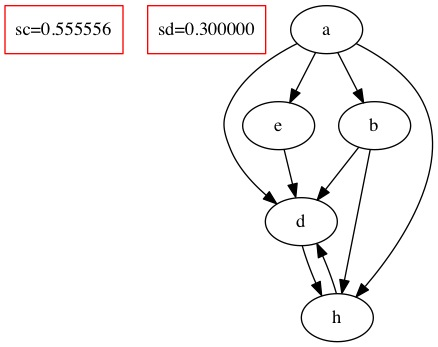
\includegraphics[scale=0.7]{partie3/graph_5_9_3_10.jpeg}
        \caption{Graphe de surclassement : sc = 5/9, sd = 3/10}
    \end{center}
\end{figure}

Lorsque nous choisissons un seuil de concordance de 5/9 et un seuil de
discordance de 3/10, nous arrivons à une solution concluante. \\

L’analyse approfondie met en évidence que la solution A domine au final la
solution E (avec les pondérations que nous avons retenues), et en même temps
domine toutes les autres. \\
La solution que nous retenons dans cette analyse multi-critère est donc la solution A. \\


\end{document}
